%\documentclass[twoside,twocolumn,spanish]{article}
\documentclass{article}
\usepackage[T1]{fontenc}
\usepackage[utf8]{inputenc}
\usepackage{graphicx}
\usepackage[spanish]{babel}
\usepackage{amssymb,amsmath,geometry,multicol,spalign,hyperref}
\setlength\columnsep{20pt}
\usepackage[usenames,dvipsnames]{xcolor}
\usepackage{tikz,mathtools}
\usepackage{circuitikz}
\usepackage{pgfplots}
\pgfplotsset{width=5cm,compat=1.12}
\usepgfplotslibrary{fillbetween}

\title{Descarga de un condensador}
\author{Andoni Latorre Galarraga \\ \href{mailto:alatorre73@alumno.uned.es}{alatorre73@alumno.uned.es}}
\date{}
\begin{document}

\maketitle
\begin{abstract}
Se calcula el tiempo de media descarga de un condensador. También se calcula la constante RC de dos circuitos monitorizando el voltaje y el tiempo a medida que se descarga un condensador. El experimento se ha realizadoç siguiendo el proceso detallado en \cite{web}.
\end{abstract}

\begin{multicols}{2}

\section*{Fundamento Teórico}
\subsection*{Ley de Ohm}
\begin{center}
\begin{circuitikz}
\draw (0,0) to[ american resistor , l=$R$] (4,0) to[ short , l=$I$] (4,-1) to[ battery1 , l=$\varepsilon$ ] (0,-1) -- (0,0); 
\end{circuitikz}
\end{center}
La ley de Ohm dice que la diferencia de potencial entre ambos bornes de un conductor, $\varepsilon$, es igual al producto de la resistencia de dicho conductor, $R$, y la intensidad de la corriente, $I$.
$$
\varepsilon = I R
$$
\subsection*{Descarga de un condensador}
Para cargar un condensador es suficiente con conectarlo a una fueunte de alimentación. Una vez cargado, si se conecta a una resistencia, $R$, el condensador comienza a descargarse. El proceso de descarga se debe al paso de corriente entre las placas del condensador. En un instante de tiempo $dt$ la cantidad de carga qu pasa de una placa a otra es $I dt$ donde $I$ es la intensidad de la corriente. Este valor tiene que ser, por la conservaciñon de carga, iial al cambio de carga, $Q$,
$$
I dt = -dQ \Rightarrow \frac{dQ}{dt} = -I
$$
Por otra parte, sbemos que la carga del condensador satisface la ecucaión,
$$
Q = CV = CRI
$$
Combinando las dos ecuaciones deducidas,
$$
\frac{dQ}{dt} = -\frac{Q}{RC}
$$
La solución de la ecuación diferencial es:
$$
Q = Q_0 e^{\frac{-t}{RC}}
$$
Dividiendo entre $C$,
$$
V = V_0 e^{\frac{-t}{RC}}
$$
Podemos calcular el tiempo que tarda el condensador en llegar a la mitad de voltaje.
$$
\frac{V_0}{2} =  V_0 e^{\frac{-t}{RC}} \Rightarrow t = RC \ln 2
$$
De la ecuación de la evolución del voltaje con el tiempo, tomando logaritmos,
$$
\textcolor{blue}{\ln V} = \frac{-1}{RC} \textcolor{blue}{t} + \ln V_0
$$
obtenemos una relación lineal entre $\ln V$ y $t$ (resaltados en azul).
\section*{Dispositivo Experimental, Procedimiento y Resultados}
Montamos un circuito como se indica en el siguiente esquema.
\begin{center}
  \begin{circuitikz}
    \draw (0,1)  to[battery1, l_=$\varepsilon$]  (0,0);
    \draw (0,1) to[switch] (0,2) -- (2,2) to[capacitor, l=$C$] (2,0) -- (4,0) to[american resistor, l=$R$] (4,2) -- (6,2) -- (6,1) circle [radius = 10pt]node[circle,fill=white,minimum size=10pt]{V} (6,1) -- (6,0) -- (0,0);
    \draw (2,2) -- (4,2);
  \end{circuitikz}
\end{center}
\begin{center}
  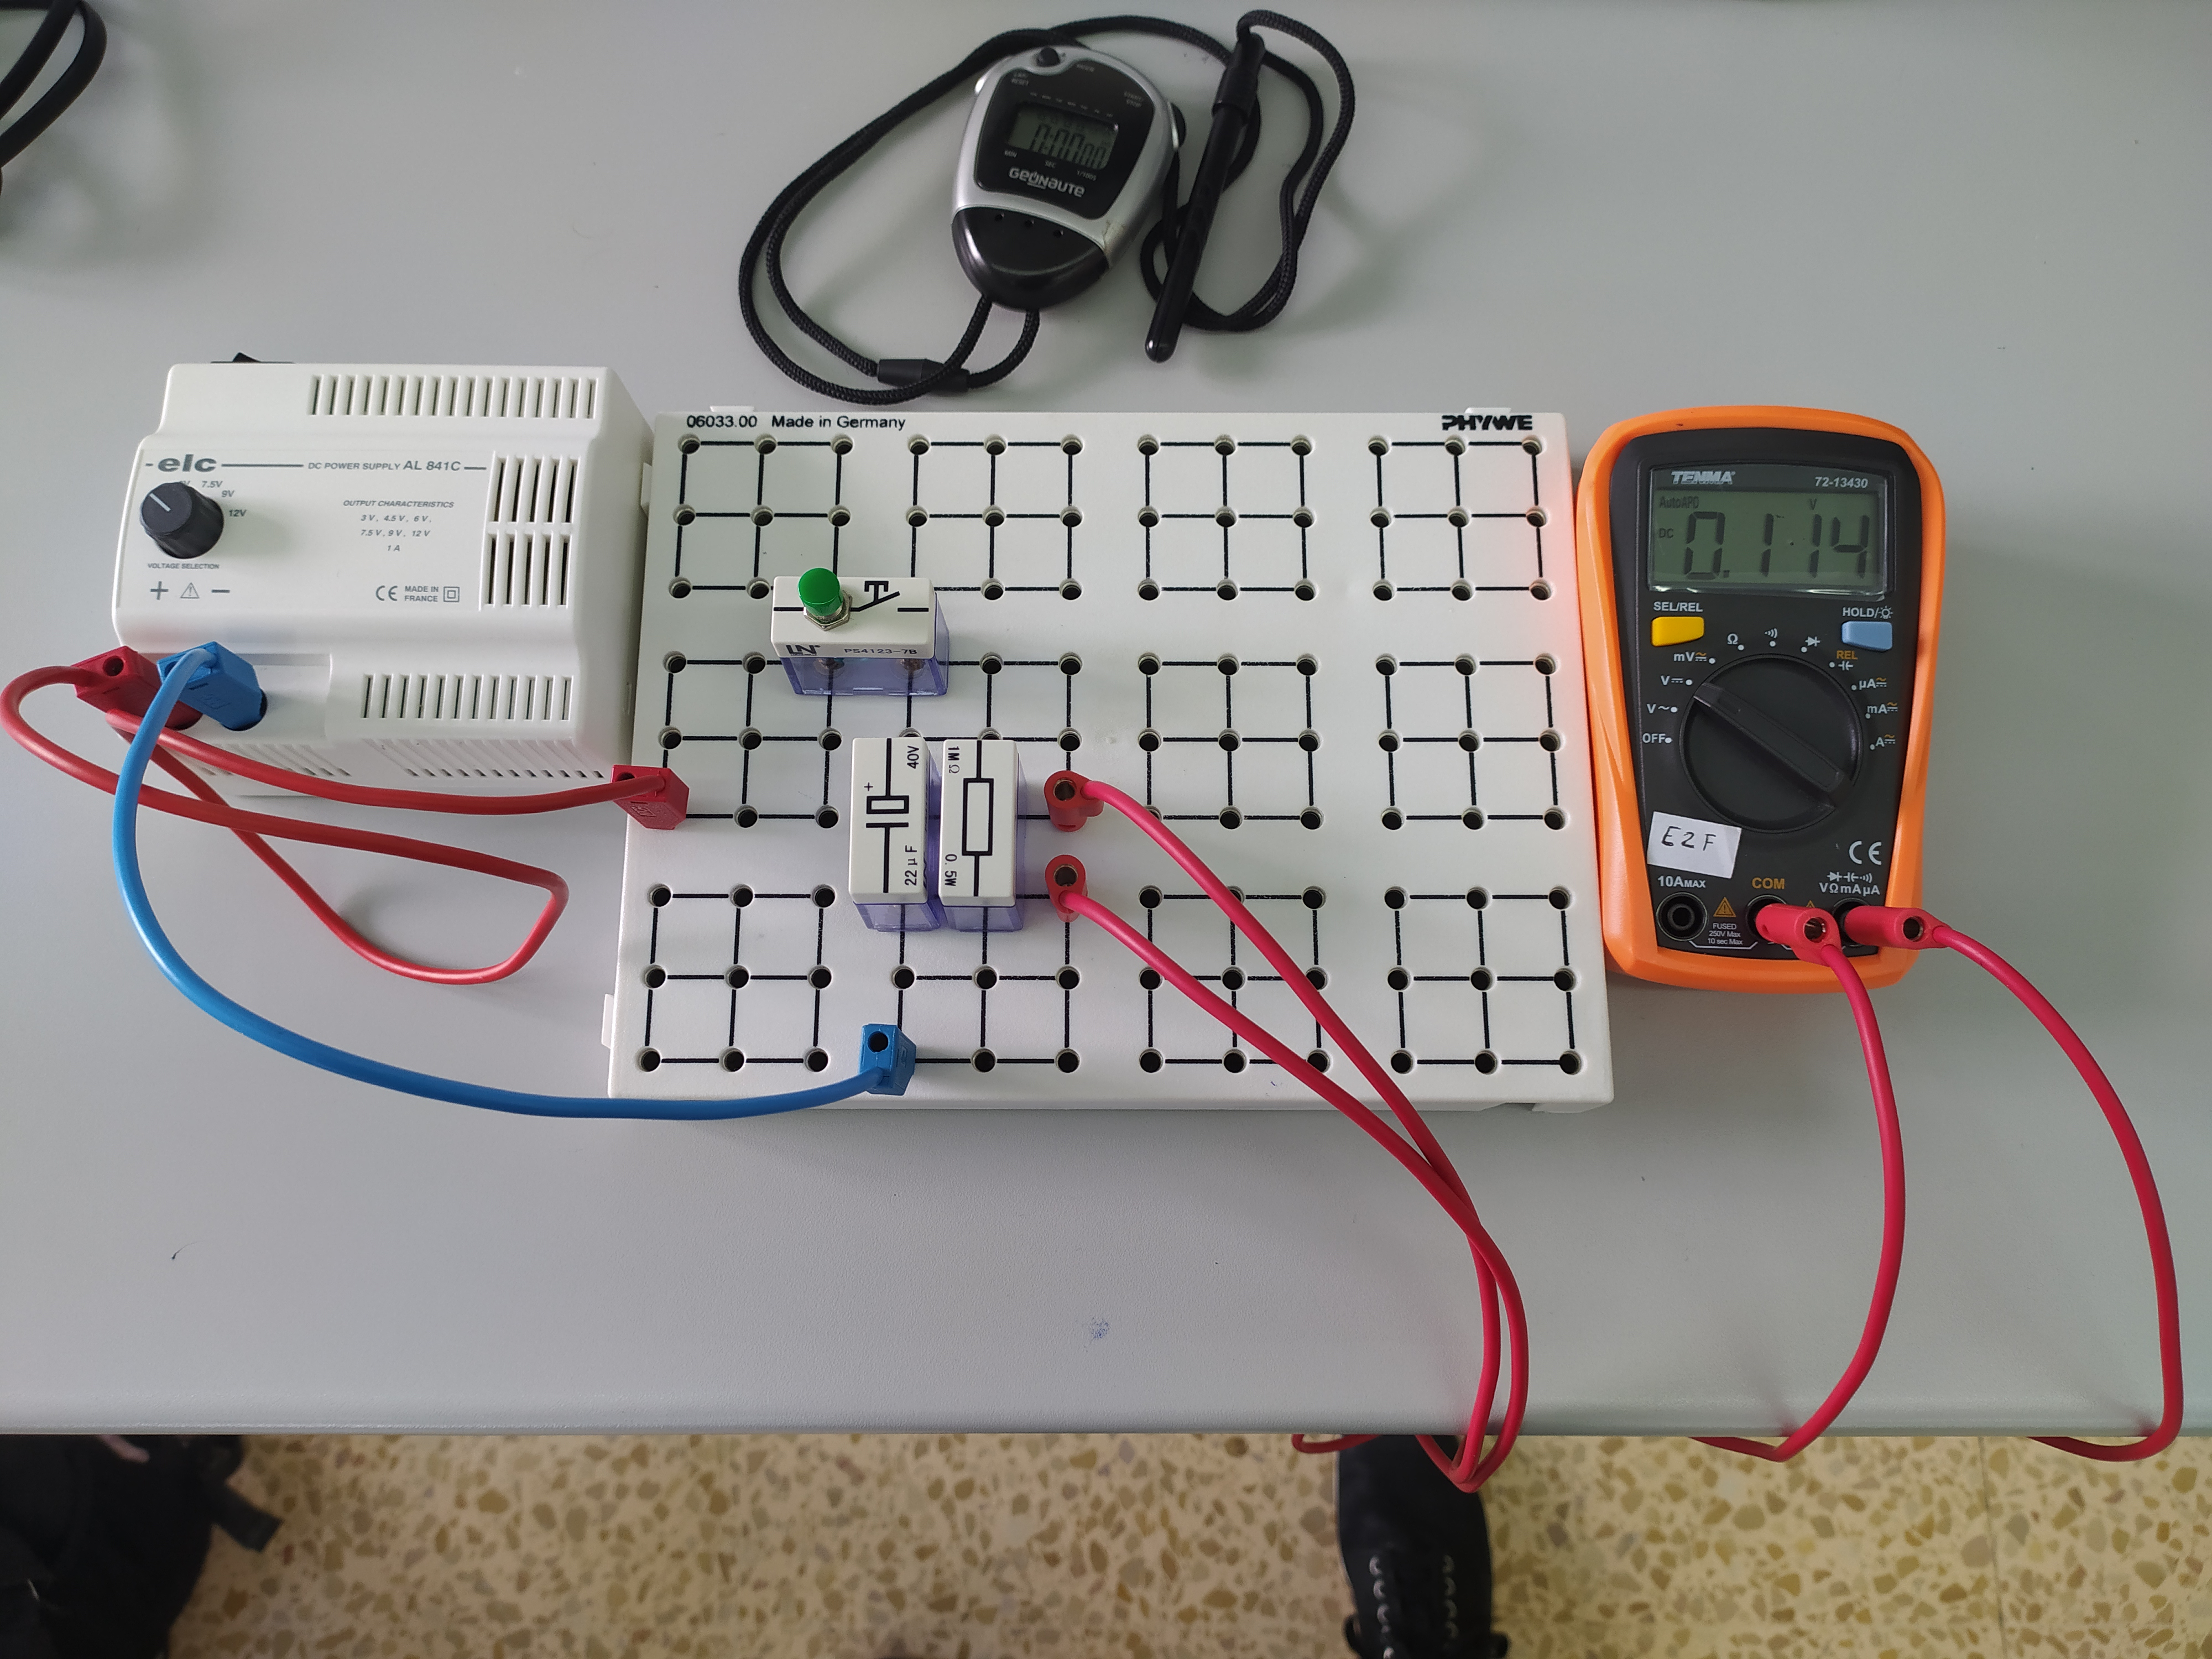
\includegraphics[width=0.45\textwidth]{figures/circuito.jpg}\\
  Figura 1: Circuito montado.

\end{center}
Hemos medido la resistencia que tenía un valor nomial de $1M\Omega$ con el multímetro. hemos obtenido $(0.997\pm 0.001)M\Omega$. También hemos tomado 4 valores de el tiempo de media descarga.
\begin{center}
Tabla 1:
$$
\begin{array}{|l|l|}\hline
  t_{1/2} \text{(s)} \\ \hline
  14.28 \\ \hline
  14.29 \\ \hline
  14.44 \\ \hline
  14.15 \\ \hline
\end{array}
$$
\end{center}
Para el error tomamos la dispersión y dividimo entre $\sqrt{4}$ como se indica en \cite{manual} p. 48-51.
$$
t_{1/2} = (14.29 \pm 0.07) \text{s}
$$
Que nos da un valor de la constante $RC$ del circuito.
$$
RC = (20.6 \pm 0.1) \text{s}
$$
Tambien hemos tomado el tiempo y el voltaje multiples veces a medida que se descarga el condensador. Los resultados obtenidos son:
\begin{center}
  Tabla 2:
  $$
  \begin{array}{|l|l|} \hline
    t\text{(s)} & V\text{(V)} \\ \hline
    2.00  & 7.98  \\ \hline
    3.82  & 7.22  \\ \hline
    5.81  & 6.39  \\ \hline
    6.06  & 6.27  \\ \hline
    8.16  & 5.53  \\ \hline
    10.06 & 5.02  \\ \hline
    12.12 & 4.46  \\ \hline
    14.29 & 4.02  \\ \hline
    15.28 & 3.70  \\ \hline
    17.01 & 3.23  \\ \hline
    18.72 & 3.05  \\ \hline
    20.09 & 2.88  \\ \hline
    22.09 & 2.61  \\ \hline
    24.19 & 2.26  \\ \hline
    26.37 & 2.03  \\ \hline
    \end{array}
  $$
\end{center}
Tomamos el logaritmo del voltaje y calculamos su error.
$$
\epsilon_{\ln V} = \frac{\epsilon_V}{V} = \frac{0.001}{V} 
$$
\begin{center}
  Tabla 3:
  $$
  \begin{array}{|l|l|l|} \hline
    t\text{(s)} & \ln V\text{(lnV)} & \epsilon_{\ln V}\text{(lnV)} \\ \hline
    2.00  & 2.07694 & 0.00013  \\ \hline
    3.82  & 1.97685 & 0.00014  \\ \hline
    5.81  & 1.85473 & 0.00016  \\ \hline
    6.06  & 1.83578 & 0.00016  \\ \hline
    8.16  & 1.71019 & 0.00018  \\ \hline
    10.06 & 1.6134  & 0.0002  \\ \hline
    12.12 & 1.4951  & 0.0002  \\ \hline
    14.29 & 1.3913  & 0.0002  \\ \hline
    15.28 & 1.3083  & 0.0003  \\ \hline
    17.01 & 1.1725  & 0.0003  \\ \hline
    18.72 & 1.1151  & 0.0003  \\ \hline
    20.09 & 1.0578  & 0.0003  \\ \hline
    22.09 & 0.9594  & 0.0004  \\ \hline
    24.19 & 0.8154  & 0.0004  \\ \hline
    26.37 & 0.7080  & 0.0005  \\ \hline
    \end{array}
  $$
\end{center}
En la siguiente figura se representa $\ln V$ frente a $t$, los errores no se representan por ser muy pequeños en relación con los valores de las medidas.
\begin{center}
  \includegraphics[width=0.45\textwidth]{figures/regresión.png}\\
  Figura 2: $\ln V$ frente a $t$ junto con la recta de regresión $y=ax+b$.
  $$
  \begin{array}{cc}
    a = (-0.0563\pm 0.0006) \text{s\textsuperscript{-1}} \\
    b = (2.180\pm 0.010) \ln(\text{V}) \\
  \end{array}
  $$
\end{center}
Ahora calculamos $RC$, $V_0$ y sus errores.
$$
RC = \frac{-1}{a} \quad \epsilon_{RC} = \frac{\epsilon_a}{a^2}
$$
$$
V_0 = e^b \quad \epsilon_{V_0} = e^b \epsilon_b
$$
Finalmente obtenemos los resultados:
$$
RC = ( 17.76\pm 0.19 ) \text{s}
$$
$$
V_0 = ( 8.85\pm 0.09 ) \text{V}
$$
Ahora repetiremos el proceso sin resitencia.
\begin{center}
  Tabla 4:
  $$
  \begin{array}{|l|l|l|l|} \hline
    t\text{(s)} & V\text{(V)} & \ln V\text{(lnV)} & \epsilon_{\ln V}\text{(lnV)} \\ \hline
     2.80 & 8.90 & 2.18605 & 0.00011  \\ \hline
    59.88 & 6.65 & 1.89462 & 0.00015  \\ \hline
     8.48 & 8.60 & 2.15176 & 0.00012  \\ \hline
    56.62 & 6.71 & 1.90360 & 0.00015  \\ \hline
    11.05 & 8.47 & 2.13653 & 0.00012  \\ \hline
    32.64 & 7.54 & 2.02022 & 0.00013  \\ \hline
    49.24 & 6.95 & 1.93874 & 0.00014  \\ \hline
     6.33 & 8.62 & 2.15409 & 0.00012  \\ \hline
    15.31 & 8.24 & 2.10900 & 0.00012  \\ \hline
    21.27 & 8.04 & 2.08443 & 0.00012  \\ \hline
    39.52 & 7.30 & 1.98787 & 0.00014  \\ \hline
    24.84 & 7.88 & 2.06433 & 0.00013  \\ \hline
    37.87 & 7.39 & 2.00013 & 0.00014  \\ \hline
    27.33 & 7.80 & 2.05412 & 0.00013  \\ \hline
    45.21 & 7.13 & 1.96431 & 0.00014  \\ \hline
    17.27 & 8.19 & 2.10291 & 0.00012  \\ \hline
    30.43 & 7.65 & 2.03471 & 0.00013  \\ \hline
    55.08 & 6.74 & 1.90806 & 0.00015  \\ \hline
    35.12 & 7.49 & 2.01357 & 0.00013  \\ \hline
    41.86 & 7.26 & 1.98238 & 0.00014  \\ \hline
    \end{array}
  $$
\end{center}
Representamos $\ln V$ frente a $t$:
\begin{center}
  \includegraphics[width=0.45\textwidth]{figures/regresión_sin.png}\\
  Figura 3: $\ln V$ frente a $t$ junto con la recta de regresión.
\end{center}
También conseguimos los valores de $RC$ y $V_0$.
$$
RC = ( 196.9 \pm 1.9 ) \text{s}
$$
$$
V_0 = ( 8.950\pm 0.016 ) \text{V}
$$
\section*{Conclusiones}
Teniendo en cuenta el valor nomial del condensador, $22\mu$F, podemos calcular la constante $RC=21.714$ s. Este valor está cerca del que hemos calculado pero difiere significativamente. Los valores de $V_0$ obtenidos se parecen entre sí aunque la barras de error no tienen puntos en común.
\begin{thebibliography}{1}

  \bibitem{manual}Manual de la asignatura. Versión 3.7

  \bibitem{web}\url{https://uned-labo.netlify.app/practicas/te/6_practica_descarga_condensador/prak6.html}

\end{thebibliography}
\end{multicols}
\end{document}